\documentclass[twoside]{article}
\usepackage[a4paper]{geometry}
\geometry{verbose,tmargin=2.5cm,bmargin=2cm,lmargin=2cm,rmargin=2cm}
\usepackage{fancyhdr}
\pagestyle{fancy}

% nastavení pisma a~češtiny
\usepackage{lmodern}
\usepackage[T1]{fontenc}
\usepackage[utf8]{inputenc}
\usepackage[czech]{babel}

% odkazy
\usepackage{url}

\usepackage{float}
% vícesloupcové tabulky
\usepackage{multirow}
\usepackage{listings}
\usepackage{xcolor}
\usepackage{amssymb}
\usepackage{gensymb}
\usepackage{bbold}
\usepackage{amsmath}
\usepackage{siunitx}
\usepackage{mathtools}
\usepackage{commath}

% vnořené popisky obrázků
\usepackage{subcaption}

% automatická konverze EPS 
\usepackage{graphicx} 
\usepackage{epstopdf}
\epstopdfsetup{update}

\graphicspath{{./images}}

% odkazy a~záložky
\usepackage[unicode=true, bookmarks=true,bookmarksnumbered=true,
bookmarksopen=false, breaklinks=false,pdfborder={0 0 0},
pdfpagemode=UseNone,backref=false,colorlinks=true] {hyperref}


% Poznámky při překladu
\usepackage{xkeyval}	% Inline todonotes
\usepackage[textsize = footnotesize]{todonotes}
\presetkeys{todonotes}{inline}{}

%https://tex.stackexchange.com/questions/2783/bold-calligraphic-typeface
\DeclareMathAlphabet\mathbfcal{OMS}{cmsy}{b}{n}

% enumerate zacina s pismenem
\renewcommand{\theenumi}{\alph{enumi}}

% smaz aktualni page layout
\fancyhf{}
% zahlavi
\usepackage{titling}
\fancyhf[HC]{\thetitle}
\fancyhf[HLE,HRO]{\theauthor}
\fancyhf[HRE,HLO]{\today}
 %zapati
\fancyhf[FLE,FRO]{\thepage}

% údaje o autorovi
\title{OTE Domácí úkol 5a - Logaritmický zesilovač}
\author{Vojtěch Michal}
\date{\today}

%customize code listing
\definecolor{codegreen}{rgb}{0,0.6,0}
\definecolor{codegray}{rgb}{0.5,0.5,0.5}
\definecolor{codepurple}{rgb}{0.58,0,0.82}
\definecolor{backcolour}{rgb}{0.95,0.95,0.92}

\lstdefinestyle{mystyle}{
    backgroundcolor=\color{backcolour},   
    commentstyle=\color{codegreen},
    keywordstyle=\color{magenta},
    numberstyle=\tiny\color{codegray},
    stringstyle=\color{codepurple},
    basicstyle=\ttfamily\footnotesize,
    breakatwhitespace=false,         
    breaklines=true,                 
    captionpos=b,                    
    keepspaces=true,                 
    numbers=left,                    
    numbersep=5pt,                  
    showspaces=false,                
    showstringspaces=false,
    showtabs=false,                  
    tabsize=2
}

\lstset{style=mystyle}

\begin{document}

\maketitle

V simulacích pro tuto úlohu byly použity ideální operační zesilovače s nulovým 
zbytkovým napětím i vstupními proudy.

\section{Statická převodní charakteristika}

\begin{figure}[h!]
    \centering
    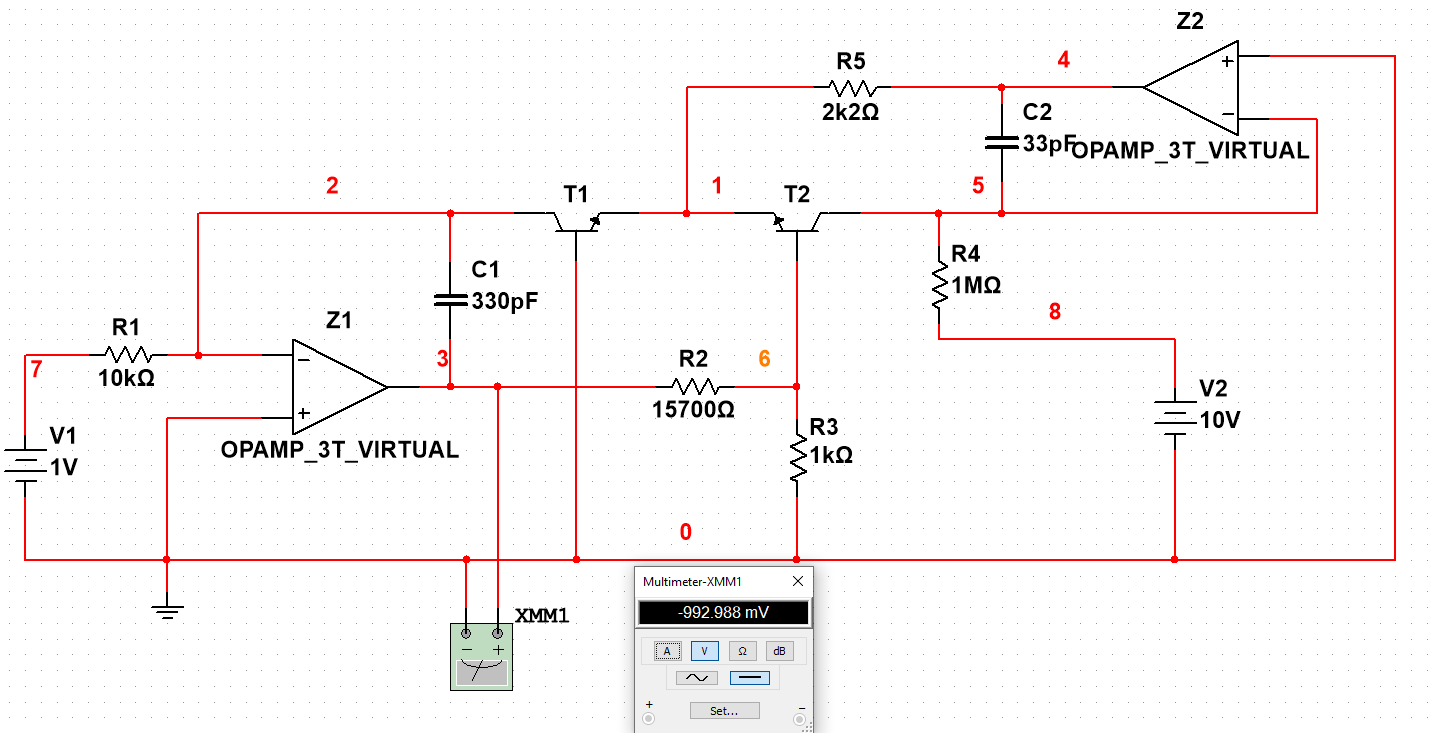
\includegraphics[width=0.65\linewidth]{staticka_schema.png}
    \caption{Schéma pro měření statické převodní charakteristiky}
    \label{fig:staticka_schema}
\end{figure}

S pomocí zapojení dle schématu \ref{fig:staticka_schema} byla změřena statická převodní charakteristika
v bodech uvedených v tabulce \ref{table:prevodni}. S použitím hodnot součástek uvedených v zadání
by měl mít logaritmický zesilovač ideální převodní charakteristiku se sklonem -1 V na dekádu.

\begin{table}[h!]
    \centering
    \begin{tabular}{c|c|c}
        Vstupní napětí $U_1$ & Výstupní napětí v uzlu 3 \\ \hline
        10 V & -1988 mV \\
        3 V & -1468 mV \\
        1 V & -992,9 mV \\
        300 mV & -473 mV \\
        100 mV & 1,57 mV \\
        30 mV & 521,6 mV \\
        10 mV & 995,9 mV \\
        3 mV & 1515 mV \\
        1 mV & 1986 mV
    \end{tabular}
    \caption{Statická převodní charakteristika logaritmického zesilovače}
    \label{table:prevodni}
\end{table}

Tytéž hodnoty jsou vykresleny na grafu \ref{fig:prevod_char}, kde je srovnána reálná (naměřená) převodní charakteristika
s tou ideální. Velikost absolutní odchylky mezi oběma je vygrafována na \ref{fig:chyba}.

\begin{figure}[h!]
    \centering
    \begin{subfigure}{0.48\textwidth}
        \centering
        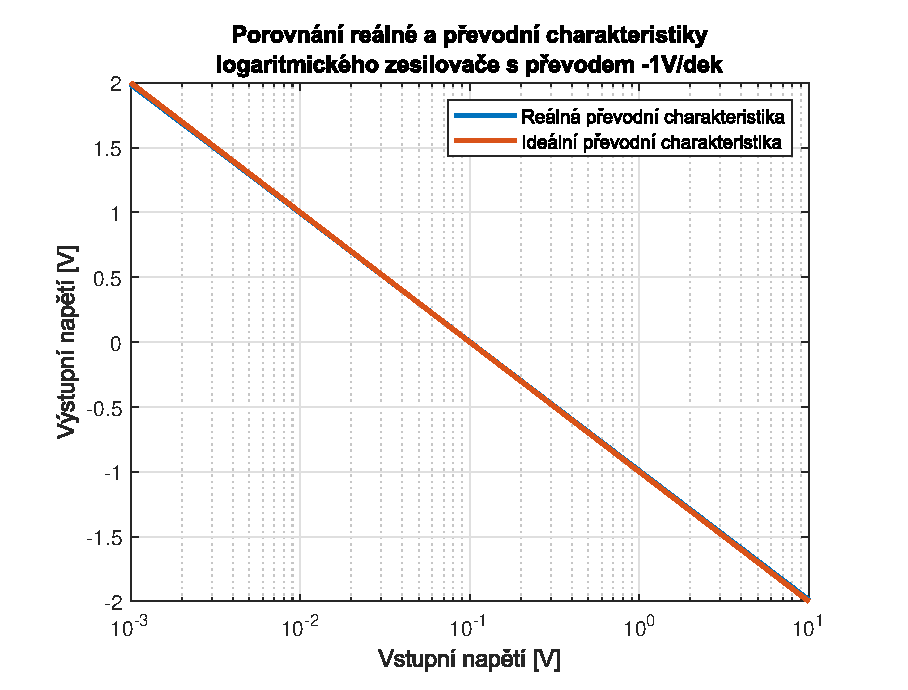
\includegraphics[width=1\linewidth]{prevod_char.eps}
        \caption{Srovnání převodních charakteristik}
        \label{fig:prevod_char}
    \end{subfigure}
    \begin{subfigure}{0.48\textwidth}
        \centering
        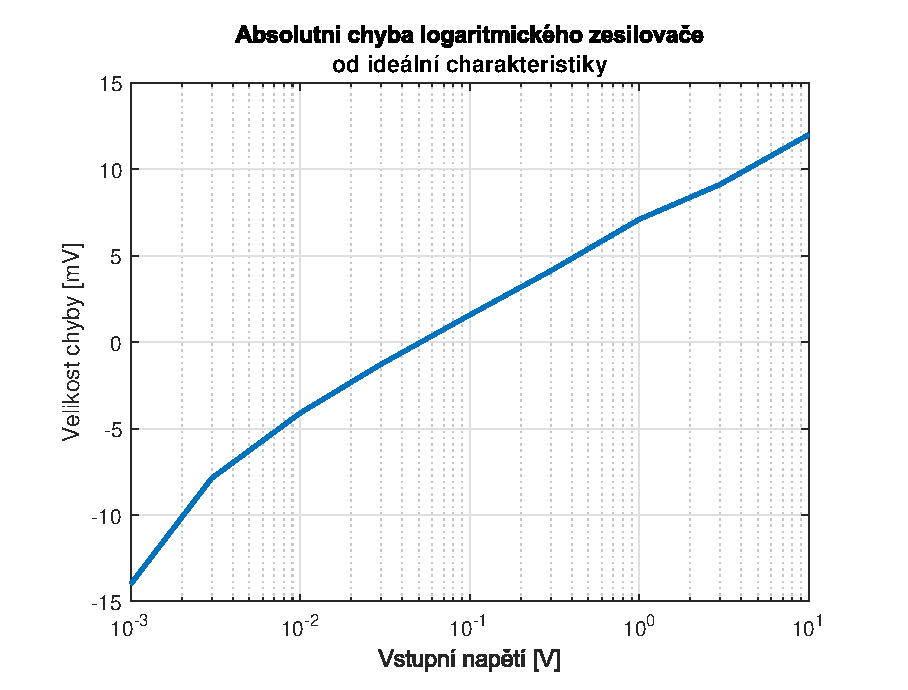
\includegraphics[width=1\linewidth]{chyba_prevodu.eps}
        \caption{Chyba reálné převodní charakteristiky}
        \label{fig:chyba}
    \end{subfigure}

    \caption{Vlastnosti přechodové charakteristiky logaritmického zesilovače}
    \label{fig:step}
\end{figure}

\section{Časový průběh odezvy na trojúhelník}

\begin{figure}[h!]
    \centering
    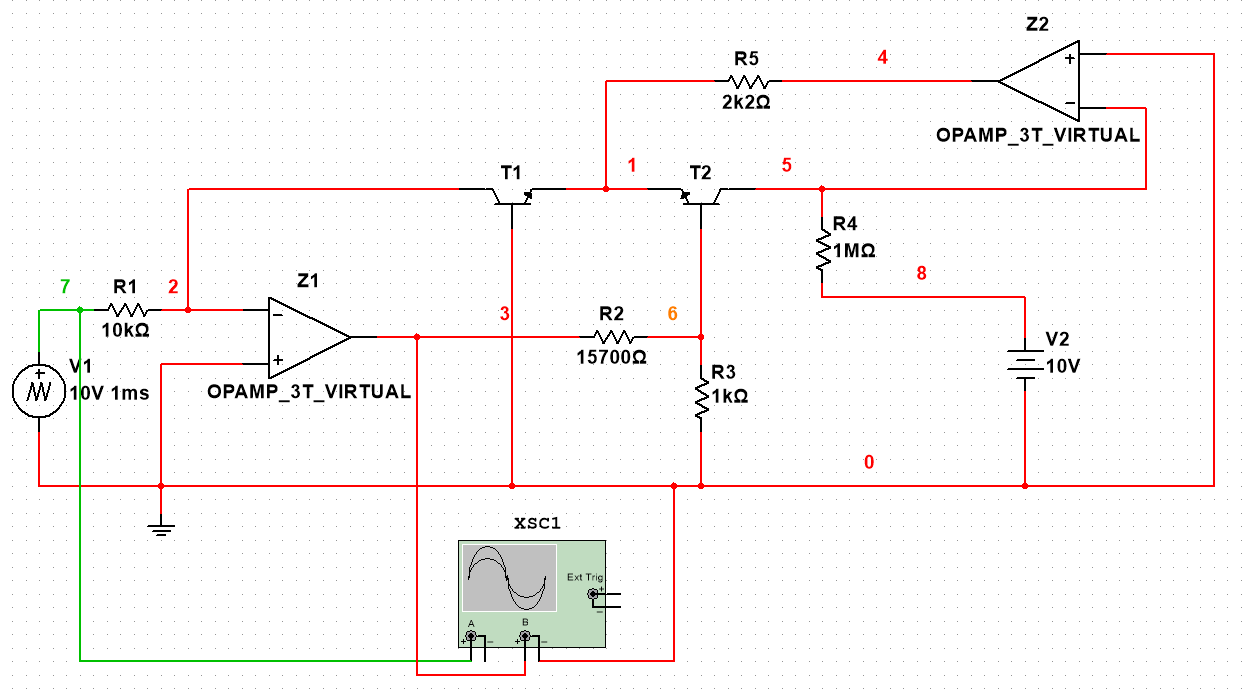
\includegraphics[width=0.65\linewidth]{prubeh_schema.png}
    \caption{Schéma pro zachycení časových průběhů odezvy na trojúhelníkový signál}
    \label{fig:prubeh_schema}
\end{figure}

Trojúhelníkový signál je po částech složen z lineárních funkcí,
na výstupu obvodu by tak měly být vidět po částech logaritmické průběhy.
Schéma zapojení je na obrázku \ref{fig:prubeh_schema}, samotné zachycené 
průběhy na obrázku \ref{fig:prubeh}.
Doba, kdy je výstup logaritmického zesilovače poblíž napětí -2 V trvá
mnohem déle než kratičký okamžik, kdy se trojúhelníkový vstup přiblíží k nule
(a na výstupu zesilovače by měly být 2 V), takže tento okemžik není na časovém průběhu
ani pořádně viditelný.

\begin{figure}[h!]
    \centering
    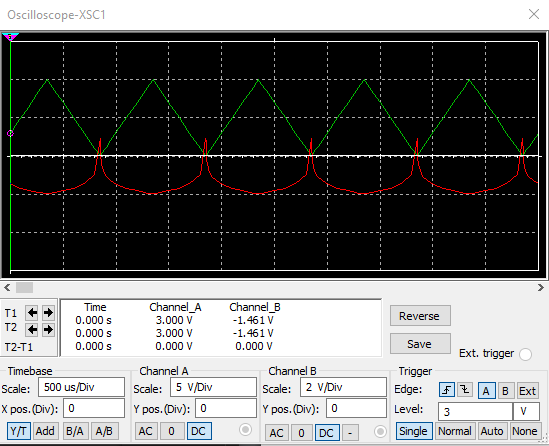
\includegraphics[width=0.65\linewidth]{prubeh.png}
    \caption{Časový průběh odezvy na trojúhelníkový vstup}
    \label{fig:prubeh}
\end{figure}




\end{document}

